\documentclass[a4paper]{article}

\usepackage{fullpage} % Package to use full page
\usepackage{parskip} % Package to tweak paragraph skipping
\usepackage{tikz} % Package for drawing
\usepackage{amsmath}
\usepackage{hyperref}
\usepackage{enumerate}
\usepackage{xcolor}
\usepackage{graphicx}
\usepackage[english,main=greek]{babel}
\usepackage[utf8x]{inputenc}
\usepackage[framed,numbered,autolinebreaks,useliterate]{mcode}

\babeltags{gr = greek}
\babeltags{en = english}
\newcommand{\code}[1]{\texttt{\texten{#1}}}
\newcommand{\huff}{\textit{\texten{Huffman }}}
\newcommand{\dpcm}{\textit{\texten{DPCM }}}
\newcommand{\matl}{\code{MATLAB }}



\title{\huge{\textbf{ΨΗΦΙΑΚΕΣ ΤΗΛΕΠΙΚΟΙΝΩΝΙΕΣ}}  \\ 
        \Large{Ακαδημαϊκό Έτος 2018-2019 \\
        1η Εργαστηριακή Άσκηση}}
\author{Χρήστος Γκουρνέλος \\ ΑΜ : 5744 \\ \href{mailto:cgkournelos@ceid.upatras.gr}{\texten{cgkournelos@ceid.upatras.gr}}}
\date{13 Ιανουαρίου 2019}

\begin{document}

\maketitle

\section*{Μέρος Α -- Κωδικοποίηση \huff}
    Στο πρώτο μέρος της εργασίας καλούμαστε να υλοποιήσουμε ένα σύστημα κωδικοποίησης/αποκωδικοποίησης 
    μιας πηγής χαρακτήρων κειμένου βασισμένο στον κώδικα \huff. Ειδικότερα ο κώδικας αυτός αποτελεί έναν
    βέλτιστο \textit{(ελάχιστο μέσο μήκος κώδικα)} προθεματικό κώδικα και χρησιμοποιείται ευρέως για 
    συμπίεση αρχείων ή κωδικοποίησή διαφόρων πηγών χωρίς απώλειες \textit{(\texten{lossless})}. Μέτα το
    τέλος της υλοποίησης, θα εξετάσουμε την αποτελεσματικότητα του συστήματος τόσο στην χρήση «τεχνητών»
    πηγών (τυχαία παραγόμενοι χαρακτήρες) όσο και πραγματικών πηγών (αρχείου Αγγλικών λέξεων). \textit{
    To περιβάλλον υλοποίησής και δοκιμών είναι η \matl}.
    
    Παρακάτω παρουσιάζονται αναλυτικά τα αποτελέσματα του κάθε υποερωτήματος:
    
    \subsubsection*{-- Υλοποίησή των συναρτήσεων για την κωδικοποίηση \huff}
       Στο ερώτημα αυτό υλοποιήθηκαν 3 συναρτήσεις σχετικά με την κωδικοποίηση \huff και κάποιες 
       επιπλέον βοηθητικές συναρτήσεις. Αναλυτικά:
        \begin{enumerate}[(a)]
            \item Η συνάρτηση για τον υπολογισμό των κωδικών λέξεων είναι η  
            \code{myHuffmanDict}. Παίρνει σαν όρισμα 2 διανύσματα το αλφάβητο και το
            διάνυσμα με τις πιθανότητες εμφάνισης κάθε χαρακτήρα. Στην έξοδο επιστρέφει μια δομή
            (\textit{<<λεξικό>>}) που περιέχει έναν πίνακα με τους χαρακτήρες του αλφαβήτου
            καθώς και τον πίνακα με τις αντίστοιχες κωδικές λέξεις. \newline 
            Για την ταξινόμηση μιας δομής που περιέχει παραπάνω από έναν πίνακες υλοποιήθηκε η συνάρτηση
            \code{mySortStruct}.
            \item Η συνάρτηση για την κωδικοποίηση είναι η \code{myHuffmanEnco}. Ως
            είσοδο αυτή η συνάρτηση παίρνει την συμβολοσειρά που πρέπει να κωδικοποίησή και το
            λεξικό που έχει παραχθεί από την προηγούμενη συνάρτηση. Σαν έξοδο έχει την κωδική
            ακολουθία από 0 και 1.
            \item Η συνάρτηση για την αποκωδικοποίηση είναι η \code{myHuffmanDeco}.
            Ως είσοδο αυτή η συνάρτηση παίρνει το κωδικοποιημένο σήμα και το λεξικό που
            δημιούργησε η \code{myHuffmanDict}. Στην έξοδο επιστρέφει την
            αποκωδικοποιημένη συμβολοσειρά στο κανονικό αλφάβητο. 
        \end{enumerate}
        \emph{\underline{Σημείωση:} Για τις παραπάνω συναρτήσεις θα βρείτε το κώδικα στο Παράρτημα Α, καθώς
        και τα \texten{".m"} αρχεία στον φάκελο} \code{"../matlab/huffman"}.
    \subsubsection*{-- Επαλήθευση κωδικοποίησης για τις πηγές Α και Β}
        Σε συνέχεια της υλοποίησης του συστήματος κωδικοποίησης \huff εξετάζεται η ορθότητα του για 2
        διαφορετικές πηγές \textbf{A} και \textbf{B}.
    \begin{table}[h!]
        \centering
            \begin{tabular}{|c | c|}
                \hline
                Γράμμα & Πιθανότητα εμφάνισης \\
                \hline
                \texten{a} & 0.0817\\
                \texten{b} & 0.0149\\
                \texten{c} & 0.0278\\
                \texten{d} & 0.0425\\
                \texten{e} & 0.1270\\
                \texten{f} & 0.0223\\
                \texten{g} & 0.0202\\
                \texten{h} & 0.0609\\
                \texten{i} & 0.0697\\
                \texten{j} & 0.0015\\
                \texten{k} & 0.0077\\
                \texten{l} & 0.0403\\
                \texten{m} & 0.0241\\
                \texten{n} & 0.0675\\
                \texten{o} & 0.0751\\
                \texten{p} & 0.0193\\
                \texten{q} & 0.0095\\
                \texten{r} & 0.0599\\
                \texten{s} & 0.0633\\
                \texten{t} & 0.0906\\
                \texten{u} & 0.0276\\
                \texten{v} & 0.0097\\
                \texten{w} & 0.0236\\
                \texten{x} & 0.0015\\
                \texten{y} & 0.0197\\
                \texten{z} & 0.0074\\
                \hline
            \end{tabular} 
            \caption{ Πιθανότητές εμφάνισης γραμμάτων στην Αγγλική γλώσσα \footnotemark } 
            \label{table:1}
        \end{table}
        \newpage \footnotetext{Τα στοιχεία προέρχονται απ’ τη \href{https://en.wikipedia.org/wiki/Letter_frequency}{\texten{Wikipedia}}.}
        \begin{itemize}
            \item[$\diamond$] Η πηγή \textbf{A}  θεωρούμε πως είναι μια τεχνητή πηγή, και πιο συγκεκριμένα 
            μια διακριτή πηγή χωρίς μνήμη που παράγει πεζούς χαρακτήρες του Αγγλικού αλφάβητου με βάση 
            συγκεκριμένες πιθανότητες. Για τις πιθανότητες αυτές χρησιμοποιήθηκαν οι τιμές εμφάνισης βάση
            του Πίνακα \ref{table:1}. Με την χρήση της συνάρτησης \code{randsrc} που παρέχει η 
            \texten{MATLAB} δημιουργήθηκε τυχαία η πηγή των 10.000 χαρακτήρων. \newline
            Παρατηρήσεις:
            \begin{enumerate}
                \item Το μέσο μήκος του κώδικα για το Αγγλικό αλφάβητο με αυτές τις πιθανότητες ισούται 
                με: \begin{center} $\overline{L}_{Α} =  4,2050$ \end{center}
                \item H μέγιστη εντροπία της πηγής με 26 χαρακτήρες ισούται με: 
                \begin{center} $H(\cdot)_{max} =  4,7004$ \end{center}
                \item Η εντροπία της πηγής \textbf{A} με αυτές τις πιθανότητες ισούται 
                με: \begin{center} $H(\cdot)_{Α} =  4,1757$ \end{center}
                \item Η αποδοτικότητα του \huff ισούται με:  
                \begin{center} $ \eta_A =  \frac{H(\cdot)_{Α}}{\overline{L}_{Α}} =  0,9930 $ \end{center}
                \item Η κωδικοποίηση και η αποκωδικοποίηση γίνεται σωστά, ελέγχοντας αν ισούται 
                το αποτέλεσμα της \code{myHuffmanDeco} με την αρχική πηγή.
                \newpage
                \item Μεγέθη αρχικής και κωδικοποιημένης ακολουθίας\footnote{Μέσος όρος 10 δοκιμών με διαφορετικές τυχαίες πηγές} για την πηγή \textbf{A}:
                \begin{table}[h!]
                \centering
                    \begin{tabular}{c c}
                        Αρχικό Μέγεθος (\texten{kB}) \footnotemark & Μέγεθος κωδ/νης ακολουθίας (\texten{kB})
                         \footnotemark \\
                        \hline
                        10 & 5,23
                    \end{tabular}
                \end{table}
                \footnotetext[3]{Tα σύμβολα της πηγής αρχικά είναι τύπου \texten{\texttt{char}} (1 \texten{Byte} = 8 \texten{bits} )}
                \footnotetext{Τα σύμβολα της κωδ/νης ακολουθίας καταλαμβάνουν 1\texten{bit} ανά χαρακτήρα στην μνήμη}
                \item Τέλος αυτό που παρατηρήθηκε είναι ότι αν στην \code{randsrc} δεν δοθεί 
                σαν όρισμα ο πίνακας πιθανοτήτων, η παραγόμενη πηγή θα έχει ίδια πιθανότητα για όλα τα σύμβολά
                $(1/26)$. Αυτή η διάφορα εκφράζεται στην κωδικοποίηση διότι πλέον έχουμε μέγεθος  
                κωδικοποιημένης πηγής περίπου ίσο με $6,8$ \texten{kB}.
            \end{enumerate}
     
            \item[$\diamond$] Η πηγή \textbf{B} είναι ένα αρχείο το οποίο δίνεται και το οποίο περιέχει 3.857 
            Αγγλικές λέξεις οι οποίες ξεκινούν από το χαρακτήρα k. Εδώ να σημειωθεί ότι στο αρχείο αυτό 
            υπήρχαν κάποια επιπλέον σύμβολα που αφαιρέθηκαν και κάποιοι κεφαλαίοι χαρακτήρες που 
            αντικαταστάθηκαν με τους αντίστοιχους πεζούς.Επίσης το αρχείο μετατράπηκε σε μια ενιαία συμβολοσειρά χωρίς του χαρακτήρες αλλαγής γραμμής, ώστε να μπορεί να δοθεί σαν είσοδο
            στις συναρτήσεις για την κωδικοποίηση \huff. Ο λόγος αυτής της τροποποίησης στην πηγή 
            \textbf{B} είναι για να μπορεί να κωδικοποιηθεί με το ίδιο λεξικό που χρησιμοποιήθηκε για την
            πηγή \textbf{Α}. \newline Παρατηρήσεις:
            \begin{enumerate}
                \item Το μέσο μήκος του κώδικα, η εντροπία και η αποδοτικότητα είναι το ίδιο με πριν 
                καθώς το αλφάβητο και οι πιθανότητες δεν άλλαξαν.
                \item Η κωδικοποίηση και η αποκωδικοποίηση γίνεται σωστά, ελέγχοντας αν ισούται 
                το αποτέλεσμα της \code{myHuffmanDeco} με την αρχική πηγή.
                \item Μεγέθη αρχικής και κωδικοποιημένης ακολουθίας για την πηγή \textbf{B}:
                \begin{table}[h!]
                \centering
                    \begin{tabular}{c c}
                        Αρχικό Μέγεθος (\texten{kB}) & Μέγεθος κωδ/νης ακολουθίας (\texten{kB})\\
                        \hline
                        29,11 & 16,93
                    \end{tabular}
                \end{table}                
            \end{enumerate}
        \end{itemize}
        \emph{\underline{Σημείωση:} Για τις παραπάνω παρατηρήσεις χρησιμοποιήθηκαν τα \texten{scripts} 
        \texttt{\texten{random\_source\_test}} και \newline \texttt{\texten{kwords\_source\_test}}
        θα βρείτε το κώδικα στο Παράρτημα Α, καθώς  και τα \texten{".m"} αρχεία στον φάκελο} 
        \texttt{\texten{"../matlab/huffman/test"}}. 
    \subsubsection*{-- Κωδικοποίηση της πηγής Β με ανανεωμένες πιθανότητες συμβολών} 
        \begin{table}[h!]
        \centering
            \begin{tabular}{|c | c|}
                \hline
                Γράμμα & Πιθανότητα εμφάνισης \\
                \hline
                \texten{a} & 0.0872\\
                \texten{b} & 0.0147\\
                \texten{c} & 0.0229\\
                \texten{d} & 0.0227\\
                \texten{e} & 0.1053\\
                \texten{f} & 0.0068\\
                \texten{g} & 0.0201\\
                \texten{h} & 0.0278\\
                \texten{i} & 0.0905\\
                \texten{j} & 0.0020\\
                \textcolor{red}{\texten{k}} & \textcolor{red}{0.1562} \\
                \texten{l} & 0.0500\\
                \texten{m} & 0.0212\\
                \texten{n} & 0.0715\\
                \texten{o} & 0.0629\\
                \texten{p} & 0.0189\\
                \texten{q} & 0.0001\\
                \texten{r} & 0.0514\\
                \texten{s} & 0.0584\\
                \texten{t} & 0.0517\\
                \texten{u} & 0.0213\\
                \texten{v} & 0.0044\\
                \texten{w} & 0.0079\\
                \texten{x} & 0.0008\\
                \texten{y} & 0.0193\\
                \texten{z} & 0.0041\\
                \hline
            \end{tabular} 
            \caption{Πιθανότητές εμφάνισης γραμμάτων στο αρχείο \texten{kwords.txt} }
            \label{table:2}
        \end{table}
        Προτείνεται να επανυπολογιστούν οι πιθανότητες του κάθε συμβόλου για την πηγή \textbf{B} με βάση το ίδιο το αρχείο 
        \texten{kwords.txt}.Περιμένουμε, το μέσο μήκος κωδικοποίησης να είναι πιο μικρό απ’ ότι στο προηγούμενο ερώτημα, 
        αλλά και η κωδικοποιημένη ακολουθία να έχει μικρότερο μέγεθος από πριν.
        Αυτό πρέπει να συμβεί, γιατί η λογική του κώδικα \huff στηρίζεται στο ότι τα σύμβολα
        με μεγαλύτερη συχνότητα εμφάνισης θα έχουν μικρότερες κωδικές λέξεις έτσι ώστε μια ακολουθία να έχει όσο το δυνατόν
        μικρότερη κωδική απεικόνιση, αφού οι πιο συχνοί χαρακτήρες έχουν μικρότερες 
        κωδικές απεικονίσεις απ’ τους άλλους. Οι νέες πιθανότητες που προκύπτουν παρουσιάζονται στον Πίνακα \ref{table:2}. 
        Όπως φαίνεται η διαφορά στη πιθανότητα για το γράμμα \texten{"k"} είναι μεγάλη.
        \newline Παρατηρήσεις:
        \begin{enumerate}
            \item Το μέσο μήκος του κώδικα με τις νέες πιθανότητες ισούται 
            με: \begin{center} $\overline{L}_{B} =  4,0869$ \end{center}
            \item Η εντροπία της πηγής \textbf{Β} με τις νέες πιθανότητες ισούται 
            με: \begin{center} $H(\cdot)_{Β} =  4,0482$ \end{center}
            \newpage
            \item Η αποδοτικότητα του \huff για την πηγή \textbf{Β} ισούται με:  
            \begin{center} $ \eta_B =  \frac{H(\cdot)_{B}}{\overline{L}_{B}} =  0,9905$ \end{center}
            \item  Μεγέθη αρχικής και κωδικοποιημένης ακολουθίας για την πηγή \textbf{B}:
                \begin{table}[h!]
                \centering
                    \begin{tabular}{c c}
                        Αρχικό Μέγεθος (\texten{kB}) & Μέγεθος κωδ/νης ακολουθίας (\texten{kB}) \\
                        \hline
                        29.11 & 14.87
                    \end{tabular}
                \end{table}
        \end{enumerate}
        Παρόλο την μικρή μείωση που παρατηρείται στην αποδοτικότητα του \huff για τις καινούργιες
        πιθανότητες, το μέγεθος της κωδικοποιημένης πηγής που προκύπτει είναι μικρότερο σε σχέση με πριν κατά 
        2,06 \texten{kB}.
    \subsubsection*{-- Δεύτερης τάξης επέκταση της πηγής \textbf{Α}} 
        Στο υποερώτημα αυτό με τη βοήθεια της συνάρτησης \texttt{\texten{myNOrderSourceGen}}
        (βλ. Παράρτημα Α), μετατρέψαμε την πηγή \textbf{Α} σε 2ης τάξης. Πλέον αντί για 26 σύμβολα 
        αλφάβητο, υπάρχουν 676 ζεύγη χαρακτήρων με νέες πιθανότητές. Παρατηρήσεις:
        \begin{enumerate}
            \item Το μέσο μήκος του κώδικα για το Αγγλικό αλφάβητο με αυτές τις πιθανότητες ισούται 
                με: \begin{center} $\overline{L}_{Α^2} =  8,3819$ \end{center}
                \item Η εντροπία της πηγής \textbf{A} με αυτές τις πιθανότητες ισούται 
                με: \begin{center} $H(\cdot)_{Α^2} =  8,3516$ \end{center}
                \item Η αποδοτικότητα του \huff ισούται με:  
                \begin{center} $ \eta_{A^2} =  \frac{H(\cdot)_{Α^2}}{\overline{L}_{Α^2}} =  0,9964 $ 
                \end{center}
                \item  Μεγέθη αρχικής και κωδικοποιημένης ακολουθίας για την δεύτερης τάξης επέκταση της πηγή \textbf{Α}:
                    \begin{table}[h!]
                    \centering
                        \begin{tabular}{c c}
                            Αρχικό Μέγεθος (\texten{kB}) & Μέγεθος κωδ/νης ακολουθίας (\texten{kB}) \\
                            \hline
                            10 & 5.23
                        \end{tabular}
                    \end{table}
        \end{enumerate}
        Σε σχέση με την 1ης τάξης πηγή είναι αναμενόμενο οι τιμές  να είναι διπλάσιες καθώς επίσης
        από την θεωρία θα πρέπει να ισχύει η εξής ανισότητα επειδή η Α είναι πηγή χωρίς μνήμη :
        \begin{center} 
            $ H(\cdot)_{Α} \leq \frac{\overline{L}_{Α^2}}{2} \leq H(\cdot)_{Α} + \frac{1}{2} \Leftrightarrow $ \\
            $ 4,1757 \leq \frac{8,3819}{2} \leq 4,1757 + 0,5 \Leftrightarrow  $ \\
            $ 4,1757 \leq 4.1910 \leq 4,6757$
        \end{center} 
        Επίσης βελτιώθηκε και η συμπίεση κατά 1,59 \texten{kB}.
    \subsubsection*{-- Δεύτερης τάξης επέκταση της πηγής \textbf{B}} 
        Όπως και στο προηγούμενο ερώτημα, μετατρέψαμε την πηγή \textbf{B} σε 2ης τάξης.
        \begin{itemize}
            \item[$\diamond$] Αρχικά η πηγή κωδικοποιήθηκε με τις πιθανότητες όπως έχουν υπολογισθεί για την πηγή 
            \textbf{Α}. \newline Παρατηρήσεις:
            \begin{enumerate}
                \item Το μέσο μήκος του κώδικα, η εντροπία και η αποδοτικότητα είναι το ίδιο με πριν 
                καθώς το αλφάβητο και οι πιθανότητες δεν άλλαξαν.
                \item Η κωδικοποίηση και η αποκωδικοποίηση γίνεται σωστά, ελέγχοντας αν ισούται 
                το αποτέλεσμα της \texttt{\texten{myHuffmanDeco}} με την αρχική πηγή.
                \item Μεγέθη αρχικής και κωδικοποιημένης ακολουθίας για την δεύτερης τάξης επέκταση της πηγή \textbf{B}:
                \begin{table}[h!]
                \centering
                    \begin{tabular}{c c}
                        Αρχικό Μέγεθος (\texten{kB}) & Μέγεθος κωδ/νης ακολουθίας (\texten{kB})\\
                        \hline
                        29,11 & 16,80
                    \end{tabular}
                \end{table}                            
            \end{enumerate}
            \item[$\diamond$] Στην συνέχεια η πηγή κωδικοποιήθηκε χρησιμοποιώντας τις πιθανότητες των ζευγών χαρακτήρων απ’
            το αρχείο kwords. Το νέο αλφάβητο περιέχει μόνο τα ζευγάρια που υπάρχουν στο αρχείο συνοδευόμενα με τις 
            πιθανότητες εμφάνισης τους.  Παρατηρήσεις:
            \begin{enumerate}
            \item Το μέσο μήκος του κώδικα για το Αγγλικό αλφάβητο με αυτές τις πιθανότητες ισούται 
                με: \begin{center} $\overline{L}_{Β^2} =  7,5389$ \end{center}
                \item Η εντροπία της πηγής \textbf{A} με αυτές τις πιθανότητες ισούται 
                με: \begin{center} $H(\cdot)_{B^2} =  7.5127$ \end{center}
                \item Η αποδοτικότητα του \huff ισούται με:  
                \begin{center} $ \eta_{B^2} =  \frac{H(\cdot)_{B^2}}{\overline{L}_{B^2}} =  0,9965 $ 
                \end{center}
                \item  Μεγέθη αρχικής και κωδικοποιημένης ακολουθίας για την δεύτερης τάξης επέκταση της πηγή \textbf{B}:
                    \begin{table}[h!]
                    \centering
                        \begin{tabular}{c c}
                            Αρχικό Μέγεθος (\texten{kB}) & Μέγεθος κωδ/νης ακολουθίας (\texten{kB}) \\
                            \hline
                            29,11 & 13,71
                        \end{tabular}
                    \end{table}
        \end{enumerate}
        \end{itemize}
        Συγκρίνοντας τα στοιχεία απ’ τους δύο τελευταίους πίνακες, κατ’ αρχάς παρατηρούμε
        ότι το μέσο μήκος έχει μειωθεί, λόγω του ότι οι πιθανότητες προκύπτουν απ’ το ίδιο το
        αρχείο. Στη συνέχεια βλέπουμε ότι η συμπίεση είναι καλύτερη στη δεύτερη περίπτωση με
        διαφορά 3,09 \texten{kB}.
\section*{Μέρος B -- Κωδικοποίηση Διακριτής Πηγής με τη μέθοδο \texten{DPCM}}
    Στο δεύτερο μέρος της εργασίας θα μελετήσουμε ένα σύστημα κωδικοποίησης \dpcm όπως φαίνεται στο 
    Σχήμα \ref{fig:dpcm_sys}.
    \begin{figure}[!h]
        \centering
        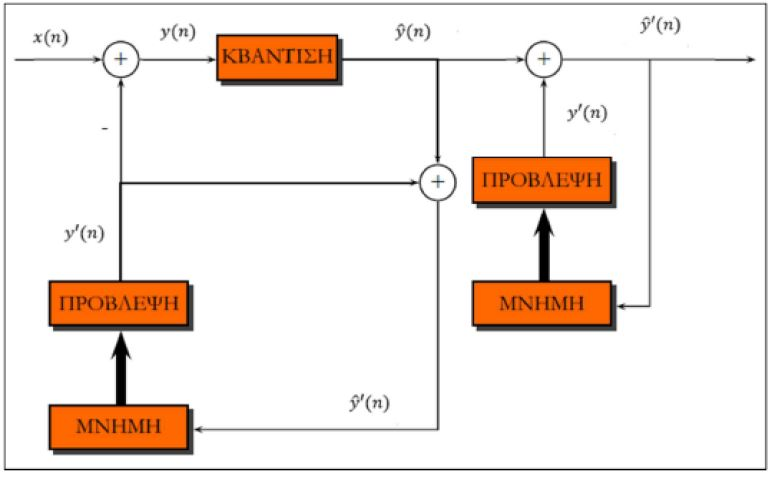
\includegraphics[width=0.7\textwidth]{figures/dpcm_system.jpg}
        \caption{Κωδικοποιητής και ο αποκωδικοποιητής ενός συστήματος \dpcm }
        \label{fig:dpcm_sys}
    \end{figure}
    \subsubsection*{--  Υλοποίηση συστήματος κωδικοποίησης/αποκωδικοποίησης \dpcm}
        Η υλοποίηση έγινε, όπως και στο πρώτο μέρος στο περιβάλλον της \matl. Τα σχετικά αρχεία κώδικα 
        παρουσιάζονται στο Παράρτημα B και βρίσκονται στον φάκελο \texttt{\texten{"../matlab/dpcm"}}.
        Αναλυτικά:
        \begin{enumerate}[(a)]
            \item Για τον υπολογισμό των συντελεστών $\alpha_i$ του φίλτρου πρόβλεψης δημιουργήθηκε η συνάρτηση  
            \\ \texttt{\texten{my\_predictor\_factors}}. Για το υπολογισμό αυτών χρησιμοποιήθηκε το κριτήριο 
            ελαχιστοποίησης του μέσου τετραγωνικού σφάλματος ανάμεσα στο εκάστοτε τρέχον δείγμα εισόδου και την 
            πρόβλεψή του. 
            \item Ο ομοιόμορφος Κβαντιστής υλοποιήθηκε με την συνάρτηση  
            \texttt{\texten{my\_quantizer}}, όπως  αναφέρεται στην εκφώνηση.
            \item Για την προσομοίωση του \dpcm συστήματος (βλ. Σχήμα \ref{fig:dpcm_sys}), φτιάχτηκαν
            δυο διαφόρετικες συναρτήσεις για τον πομπό (\texttt{\texten{my\_dpcm\_trans}}) και για 
            τον δέκτη (\texttt{\texten{my\_dpcm\_rec}}). Κάποιες παραδοχές που αξίζει να σημειωθούν 
            είναι οι εξής:
            \begin{itemize}
                \item[\texten{i}.] Για την αρχικοποίηση του συστήματος θεωρήθηκε ότι οι $p$ πρώτες 
                τιμές \textit{(μέγεθος φίλτρου)} μεταδίδονται χωρίς σφάλματα.
                \item[\texten{ii}.] Οι συντελεστές στο φίλτρο πρόβλεψης θα κβαντίζονται στην 
                δυναμική περιοχή $[-2,2]$ σε 256 επίπεδα. O υπολογίσιμος και η κβάντιση γίνεται στον 
                πομπό, και στη συνέχεια οι συντελεστές του φίλτρου πρόβλεψης κβαντίζονται και 
                αποστέλλονται στο δέκτη.
            \end{itemize}
            Και οι δυο συναρτήσεις επιστρέφουν ένα \texttt{\texten{struct}} με τις μεταβλητές που 
            συμμετέχουν στους υπολογισμούς. Ο Πικακάς \ref{table:dpcm_vars} δείχνει τον συνδυασμό των
            μεταβλητών αυτών με την σημειογραφία της εκφώνησης και του Σχήματος \ref{fig:dpcm_sys}.
            \begin{table}[h!]
            \centering
                \begin{tabular}{|c|c|}
                    \hline
                    \textbf{Μεταβλητή \matl}    & \textbf{Μαθηματικός Συμβολισμός}      \\ \hline
                    \code{x}                    & $x(n)$                                \\ \hline
                    \code{y}                    & $y(n)$                                \\ \hline
                    \code{y\_pred}              & $y'(n)$                               \\ \hline
                    \code{y\_quant}             & $\hat{y}(n)$                          \\ \hline
                    \code{y\_mem}               & $\hat{y}'(n)$                         \\ \hline
                    \code{a\_factors}           & $a_i$                                 \\ \hline
                \end{tabular}
            \caption{Αντιστοίχηση συμβολισμών με τις συναρτήσεις \matl  } 
            \label{table:dpcm_vars}
            \end{table}    
        \end{enumerate}
    \subsubsection*{--  Διαγράμματα αρχικού σήματος και σφάλματος προβλέψεις}
        Για την αξιολόγηση της απόδοσης του προβλεπτή του συστήματος \dpcm, δοκιμάστηκε για 2 τιμές του 
        $p \geq 4$ και $ Ν=1,2,3$ \texten{bits}. Συγκεκριμένα\footnotemark, επιλέχθηκαν οι τιμές $p = 4$ (βλ. Σχήμα 
        \ref{fig:dpcm_pred_error_4}) και $p = 24$ (βλ. Σχήμα \ref{fig:dpcm_pred_error_24}).    
        \footnotetext{Για την εξαγωγή των διαγραμμάτων εκτελέσαμε το \texten{script} \code{dpcm\_predict\_test.m}  }
        \begin{figure}[!h]
            \centering
            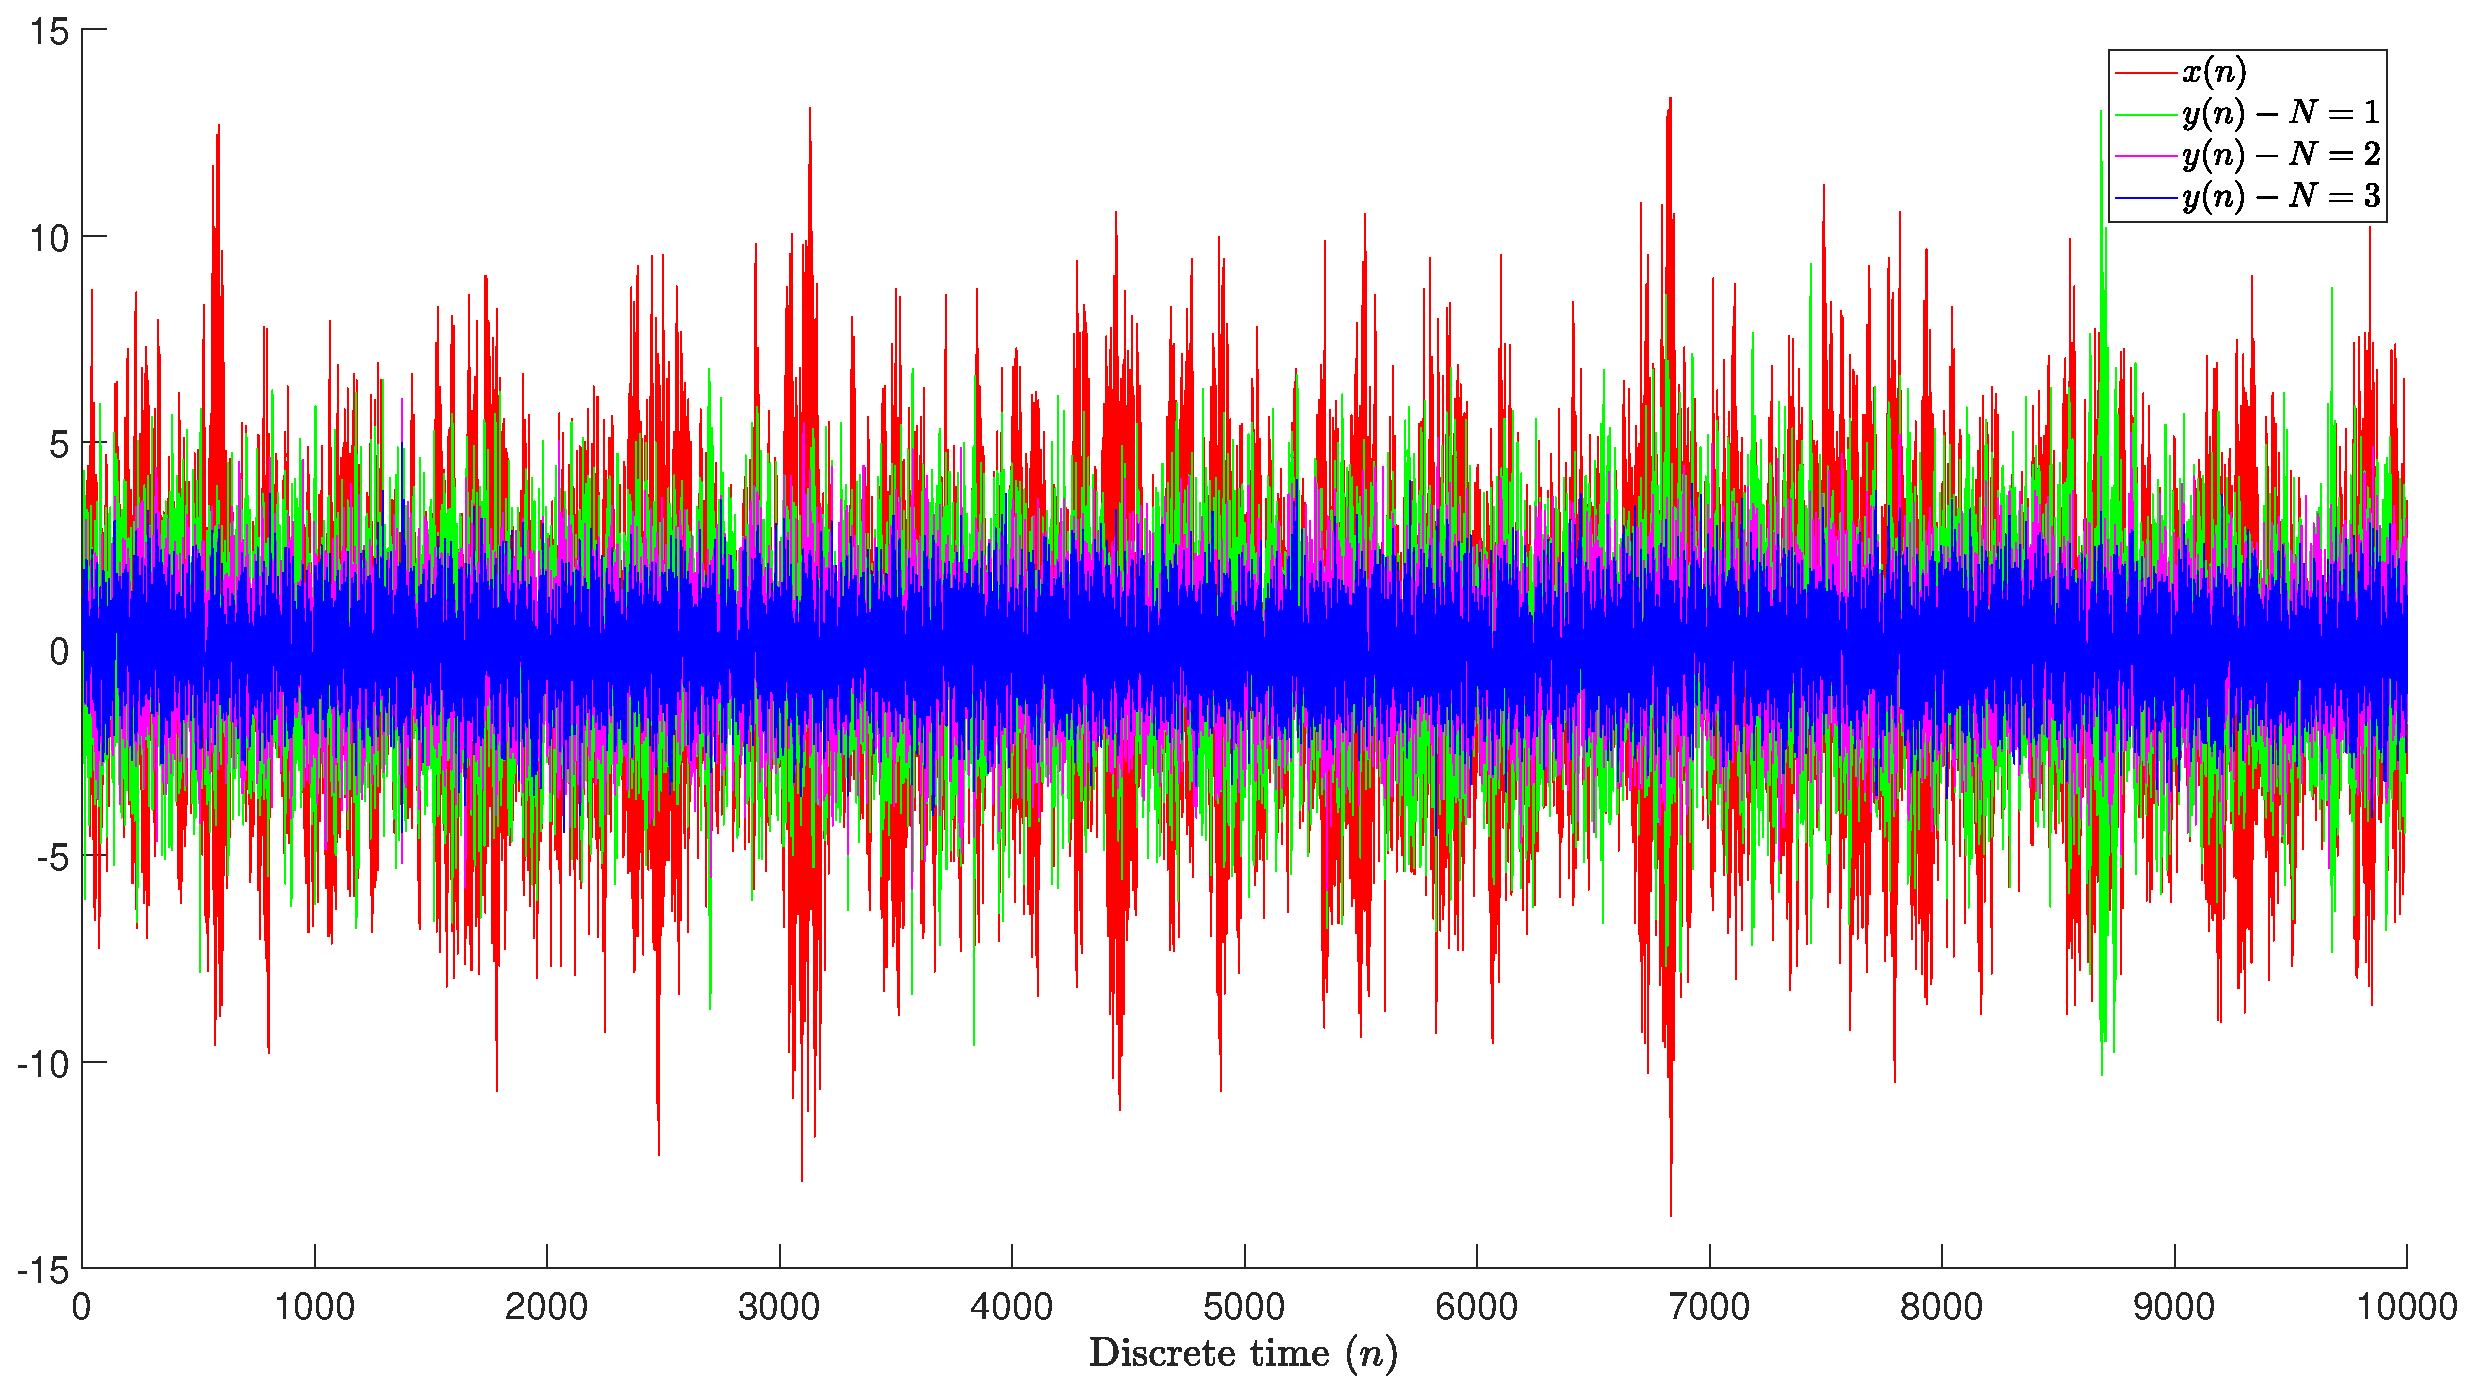
\includegraphics[width=0.95\textwidth, height = 6.5cm]{figures/dpcm_pred_error_4.eps}
            \caption{Διάγραμμα αρχικού σήματος και σφάλματος πρόβλεψης για $p = 4$ και $Ν = 1,2,3$ 
            \texten{bits}}
            \label{fig:dpcm_pred_error_4}
            \\\hspace{\textwidth}\\\hspace{\textwidth}
            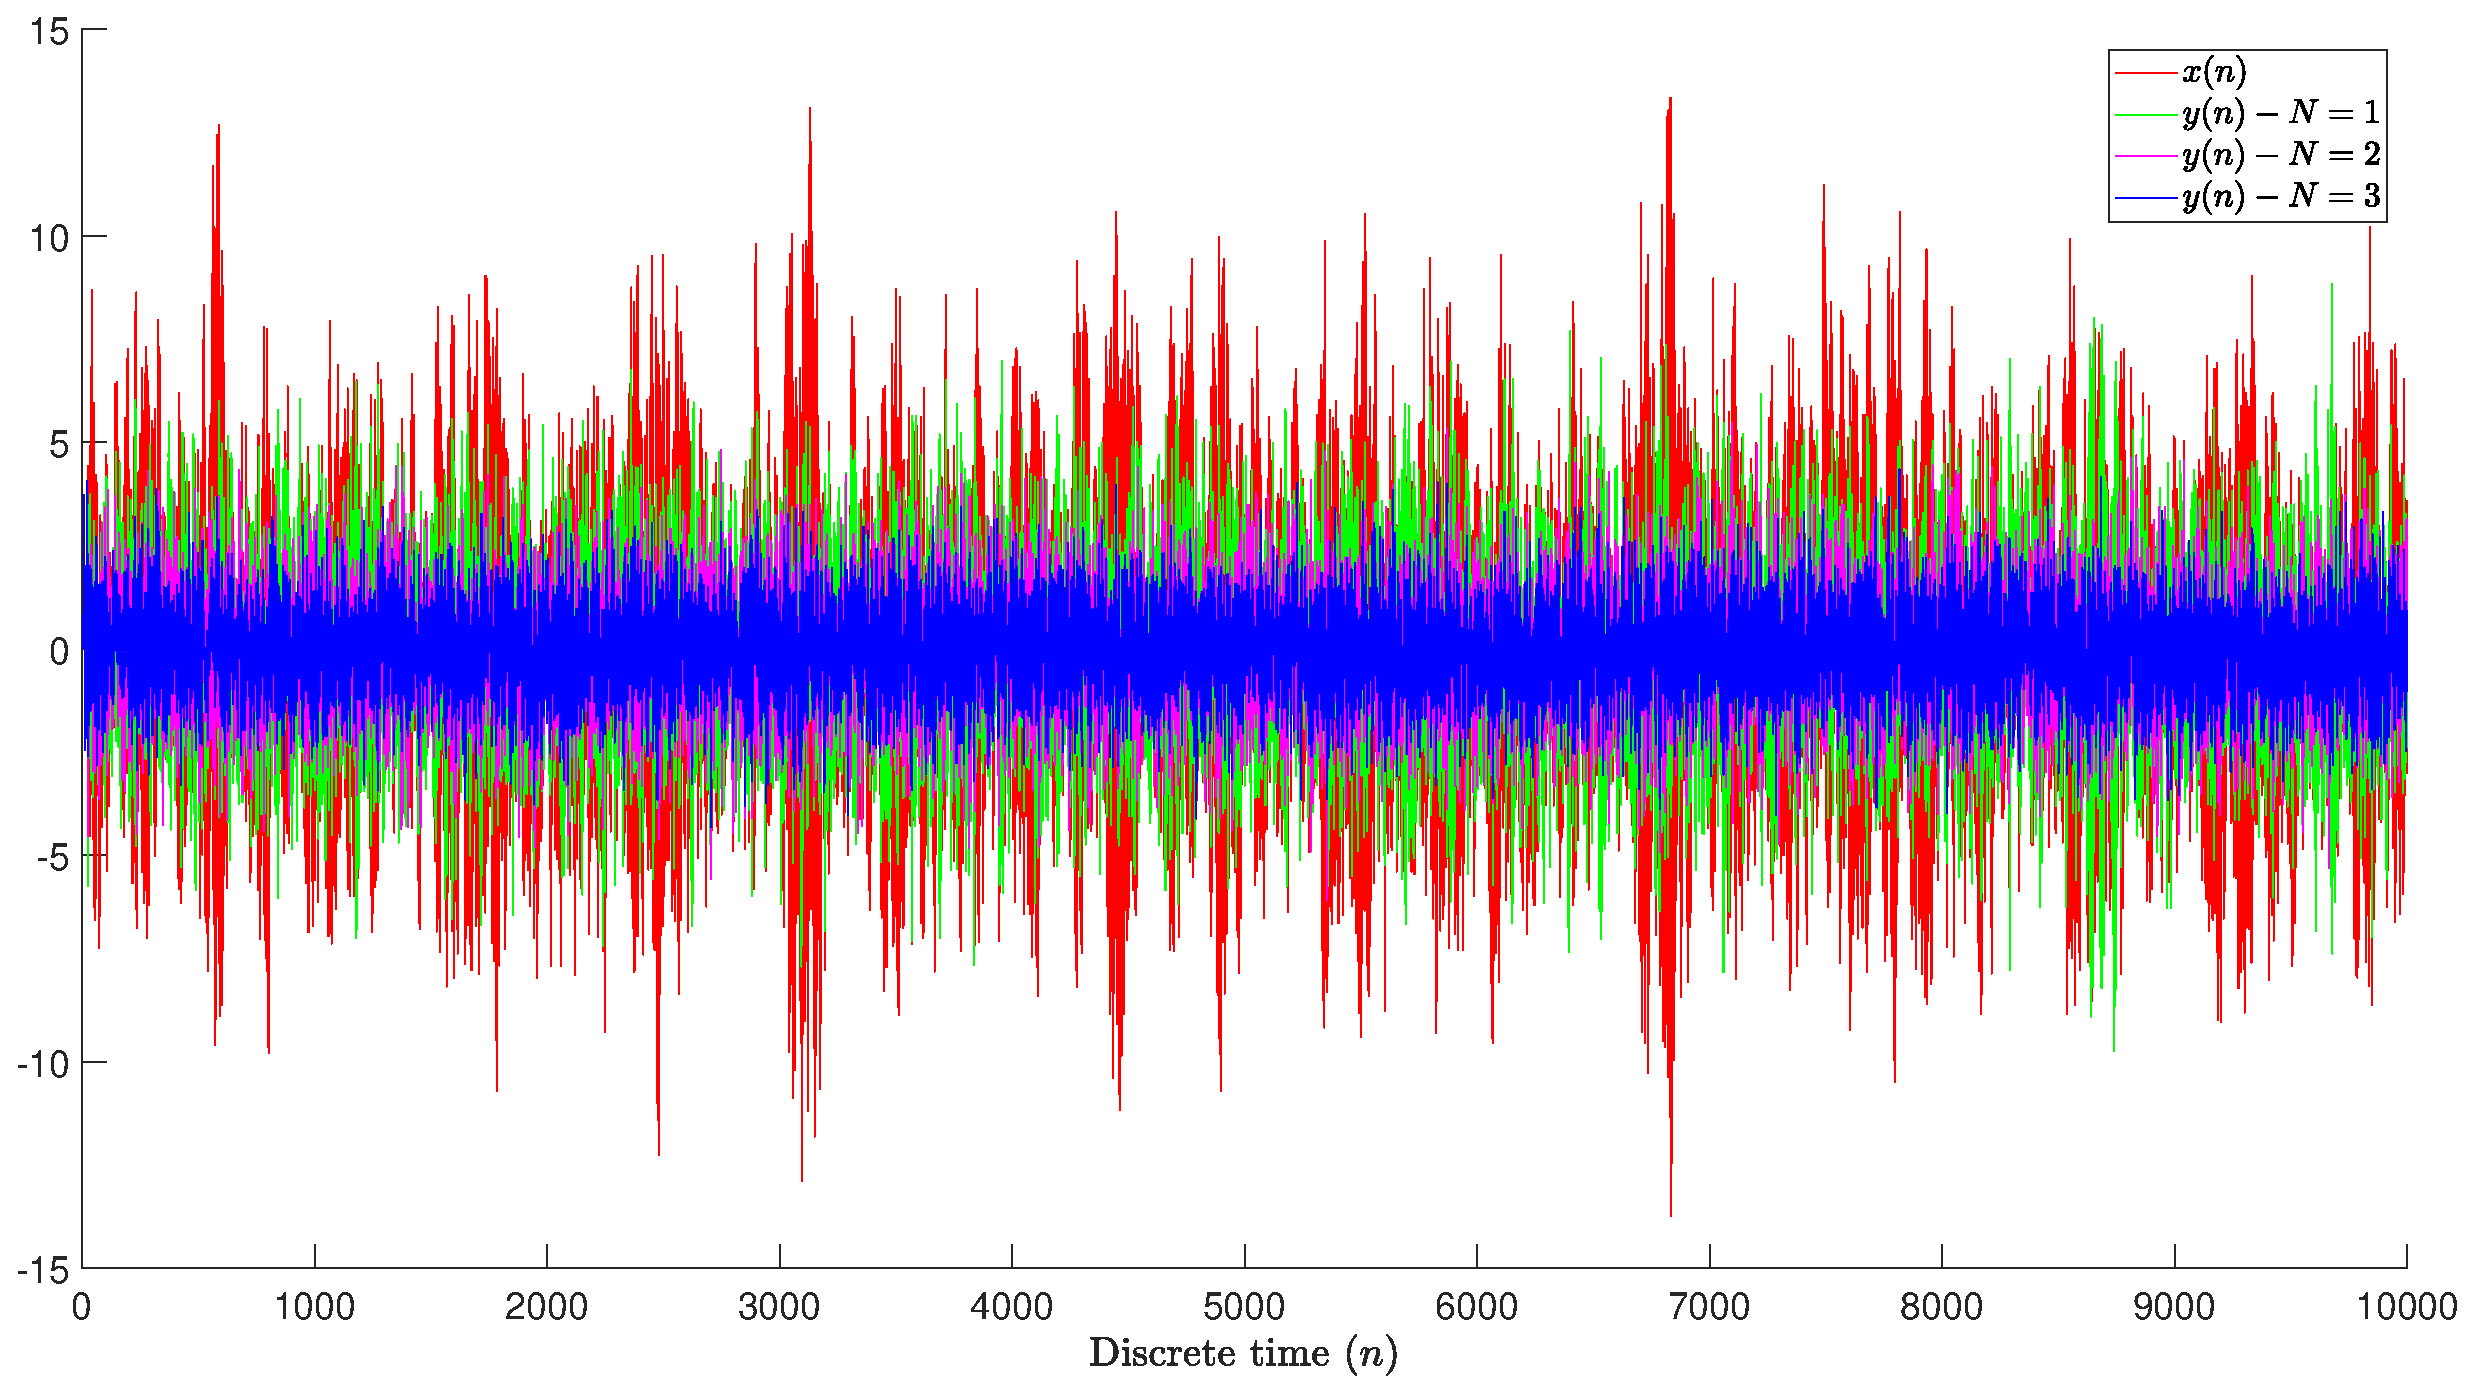
\includegraphics[width=0.95\textwidth, height = 6.5cm]{figures/dpcm_pred_error_24.eps}
            \caption{Διάγραμμα αρχικού σήματος και σφάλματος πρόβλεψης για $p = 24$ και $Ν = 1,2,3$
            \texten{bits}}
            \label{fig:dpcm_pred_error_24}
        \end{figure}      
        \\ Όπως παρατηρείται εύκολα και στα δυο διαγράμματα, όσο μεγαλώνει το $N$ το σφάλμα πρόβλεψης 
        \textit{\texten{"}στενεύει\texten{"}} δηλαδή μειώνεται. Αυτό σημαίνει ότι όσο πιο λεπτομερή κβάντιση 
        κάνουμε τόσο ελαχιστοποιείται η διαφορά του σήματος εισόδου από την πρόβλεψη. Από την πλευρά η αύξηση 
        του $p$ κατά 20 τιμές βλέπουμε ότι δεν έχει σχεδόν καμία διαφορά και καμία επίδραση στο σφάλμα 
        πρόβλεψης.
    \subsubsection*{--  Απόδοση \dpcm και μέσο τετραγωνικό σφάλμα πρόβλεψης}
        Για την καλύτερη αξιολόγηση της απόδοσης του προβλέπτη, στο διάγραμμα\footnotemark 
        του στο Σχήματος , παρουσιάζεται το το μέσο τετραγωνικό σφάλμα πρόβλεψης ως προς το $N$
        και για διάφορες τιμές του $p$.
        \footnotetext{Για την δημιουργία του διαγράμματος εκτελέσαμε το \texten{script} 
        \code{dpcm\_mean\_square\_error.m}  }
         \begin{figure}[!h]
            \centering
            $MSE = E(y^2(n)) =  E((x(n)-y'(n))^2)$
            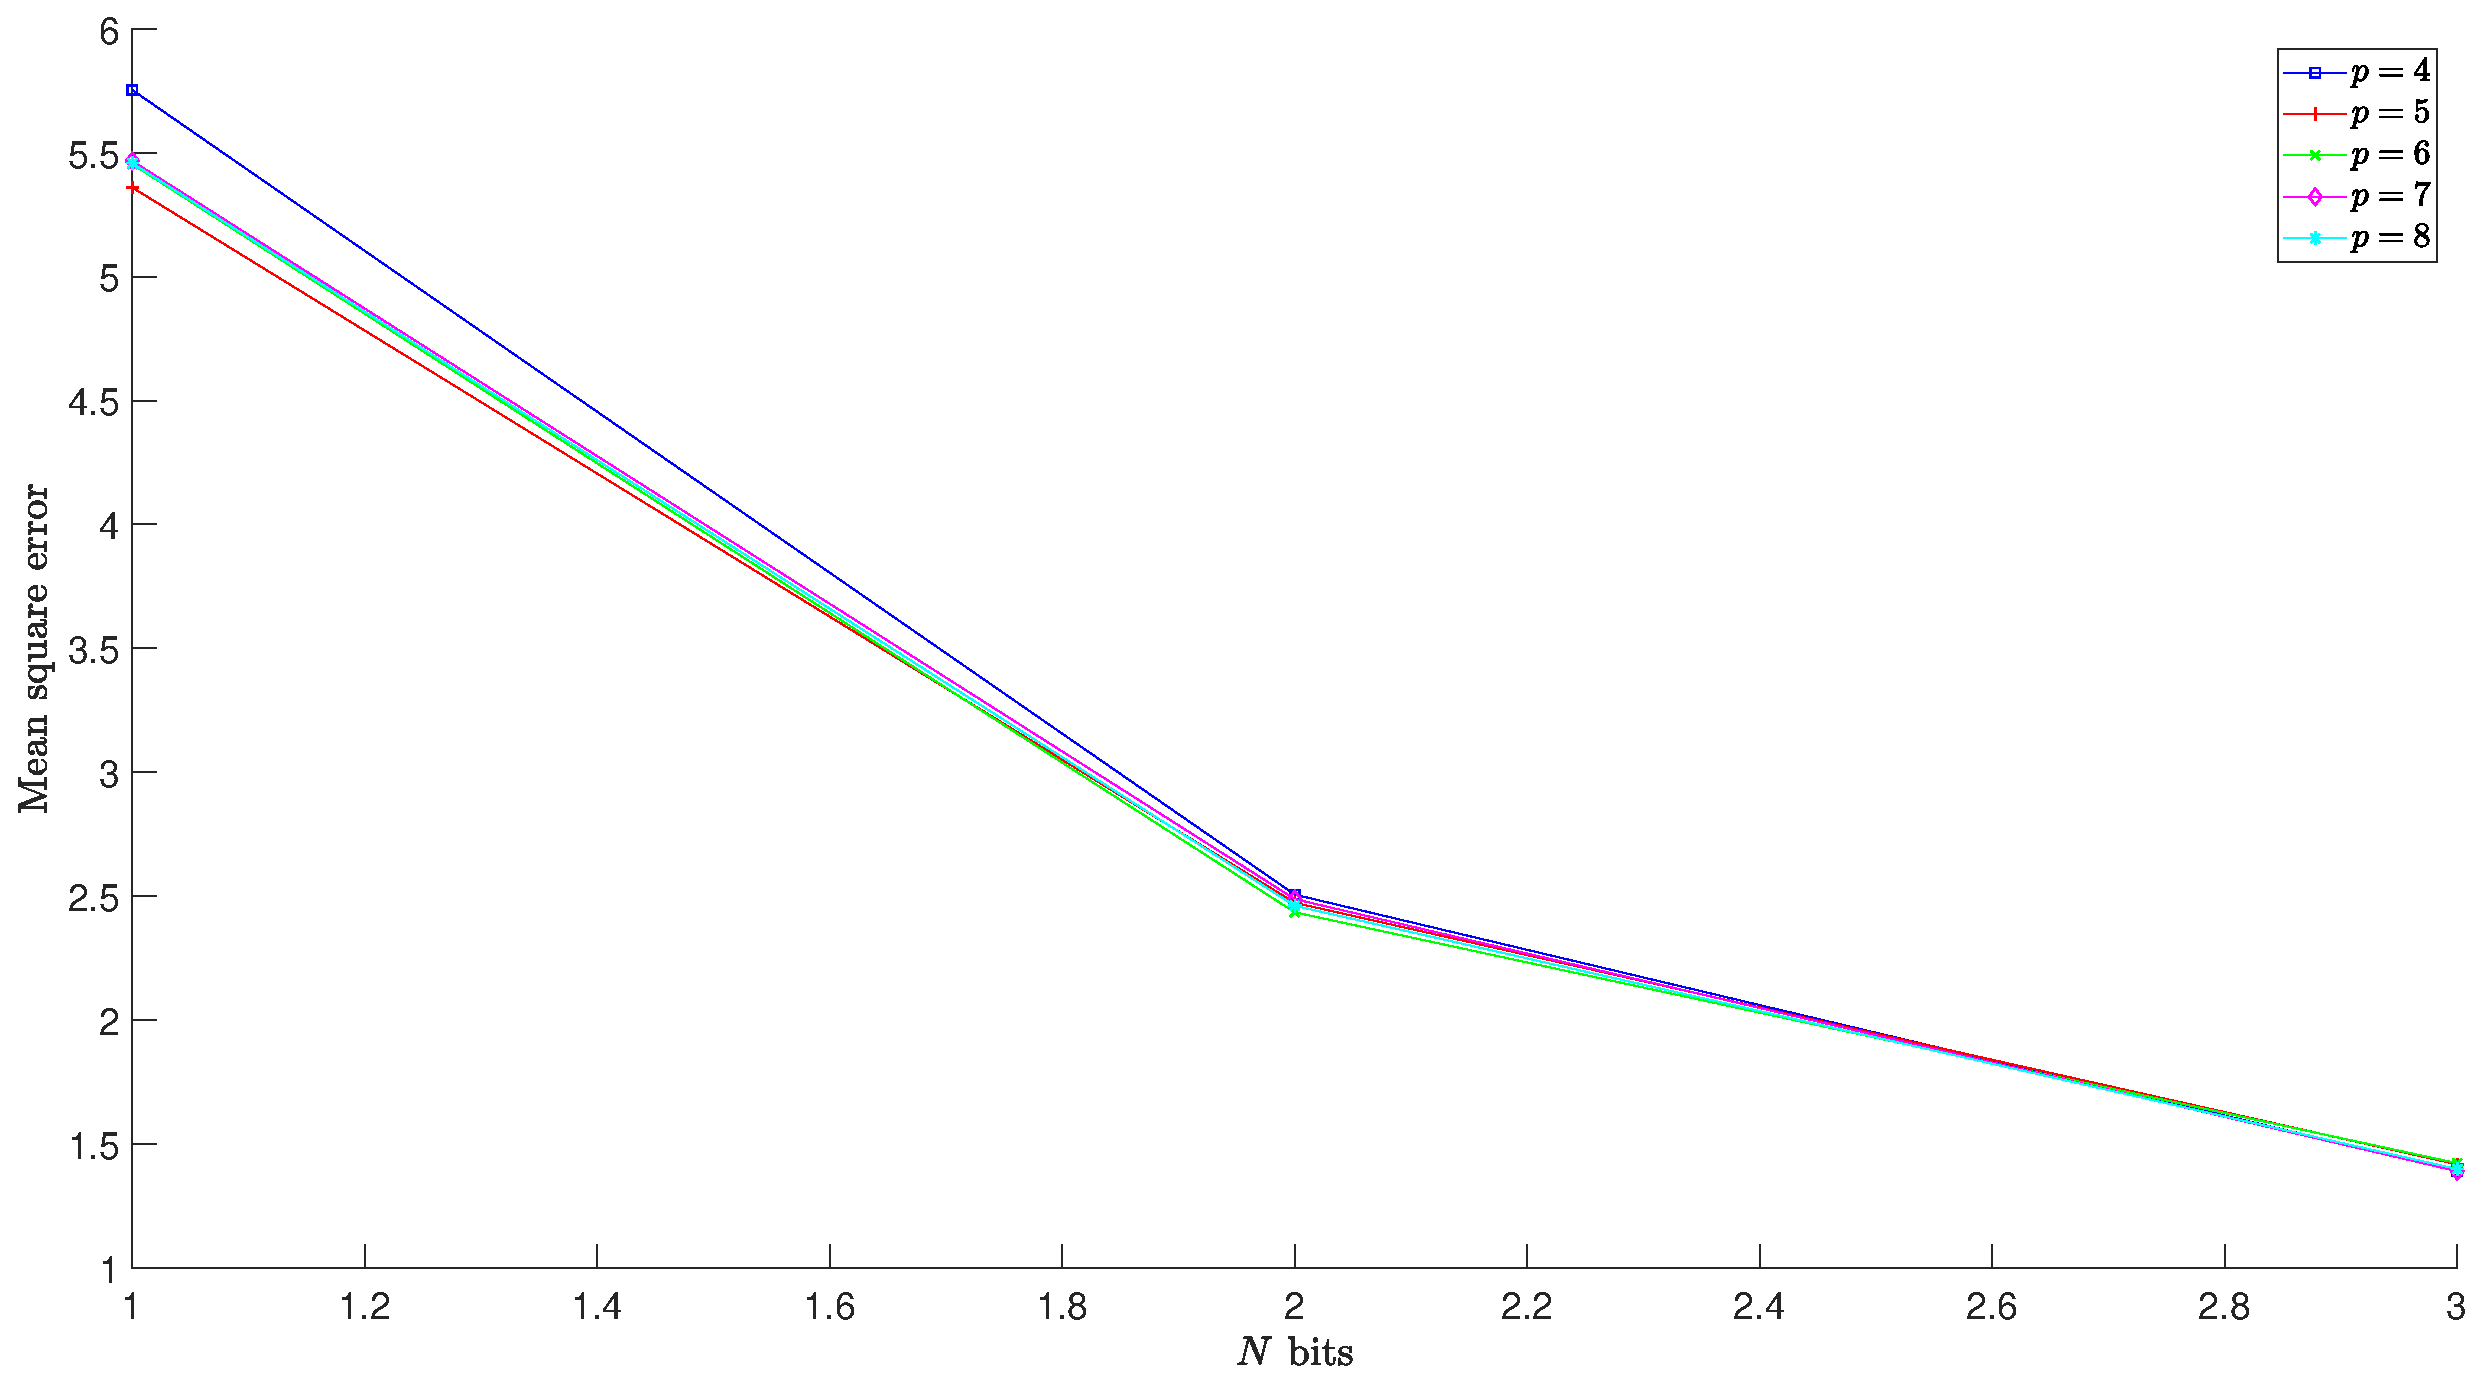
\includegraphics[width=0.95\textwidth]{figures/dpcm_mean_sq_error.eps}
            \caption{Διάγραμμα μέσου τετραγωνικού σφάλματος πρόβλεψης για ταξη προβλέπτη $p = 4:1:8$}
        \end{figure}
        Από το παραπάνω γράφημα μπορούμε να συμπεράνουμε ότι η απόδοση του φίλτρου πρόβλεψης
        του σήματος επηρεάζεται σχεδόν αποκλειστικά από την ακρίβεια κβάντισης των δειγμάτων.
        Αυτο το συμπέρασμα  προκύπτει απο το γεγονός ότι η γραφική παράσταση που σχεδιάστηκε είναι φθίνουσα σε 
        όλες τις περιπτώσεις και κάθε φορά το σφάλμα σχεδόν υποδιπλασιάζεται με την αύξηση των \texten{bits}.
        \begin{table}[h!]
            \centering
            \begin{tabular}{c  | c  | c  | c   | c}
                $p=4$       & $p=5$     & $p=6$     & $p=7$     & $p=8$     \\ 
                \hline
                1.3887	    &1.3881	    &1.3880	    &1.3879	    &1.3878     \\
                -1.5212     &-1.5185    &-1.5191    &-1.5193    &-1.5192    \\
                1.2122      &1.2087     &1.2117     &1.2109     &1.2106     \\
                -0.3016     &-0.2984    &-0.3022    &-0.2975    &-0.2998    \\
                            &-0.0025    &0.0011     &-0.0051    &0.0050     \\
                            &           &-0.0026    &0.0033     &-0.0095    \\
                            &           &           &-0.0045    &0.0073     \\
                            &           &           &           &-0.0085
            \end{tabular}
            \caption{Σεντλεστές πρόβλεψης $\alpha_i$ για κάθε τάξη $p$} 
            \label{table:a_factors}
        \end{table}
        Oι συντελεστές του φίλτρου πρόβλεψης ($\alpha_i$), παρουσιάζονται στον Πίνακα \ref{table:a_factors}.
        Παρατηρούμε ότι κυμαίνονται γύρω από το 0 και ενώ οι αρχικοί είναι σχετικά μεγάλοι αριθμοί, όσο αυξάνεται το $p$ και δημιουργούνται και άλλοι συντελεστές και σταθεροποιούνται 
        σε αριθμό τάξης $10^{-3}$.
    \subsubsection*{--  Σύγκρισή αρχικού $x(n)$ και ανακατασκευασμένου $\hat{y}'(n)$ σήματος }
        Στο ερώτημα αυτό γίνεται σύγκριση του αρχικού με το ανακατασκευασμένο σήμα. Παρακάτω παρουσιάζονται  
        τα διαγράμματα\footnotemark με το αρχικό  και  το ανακατασκευασμένο σήμα για $p=4$ και $p=8$. 
        Κάθε σχήμα αφορά διαφορετικά \texten{bits} κβάντισης $N =  1,2,3$ και για  να μπορέσουμε να 
        παρατηρήσουμε καλύτερα τις τιμές εχουμε πάρει τυχαια ενα παραθυρο 100 τιμών  \textit{(5000 - 5100)}.
        \footnotetext{Για την δημιουργία του διαγράμματος εκτελέσαμε το \texten{script} 
        \code{dpcm\_reconstruct\_signal.m}  }
        \begin{figure}[!h]
            \centering
            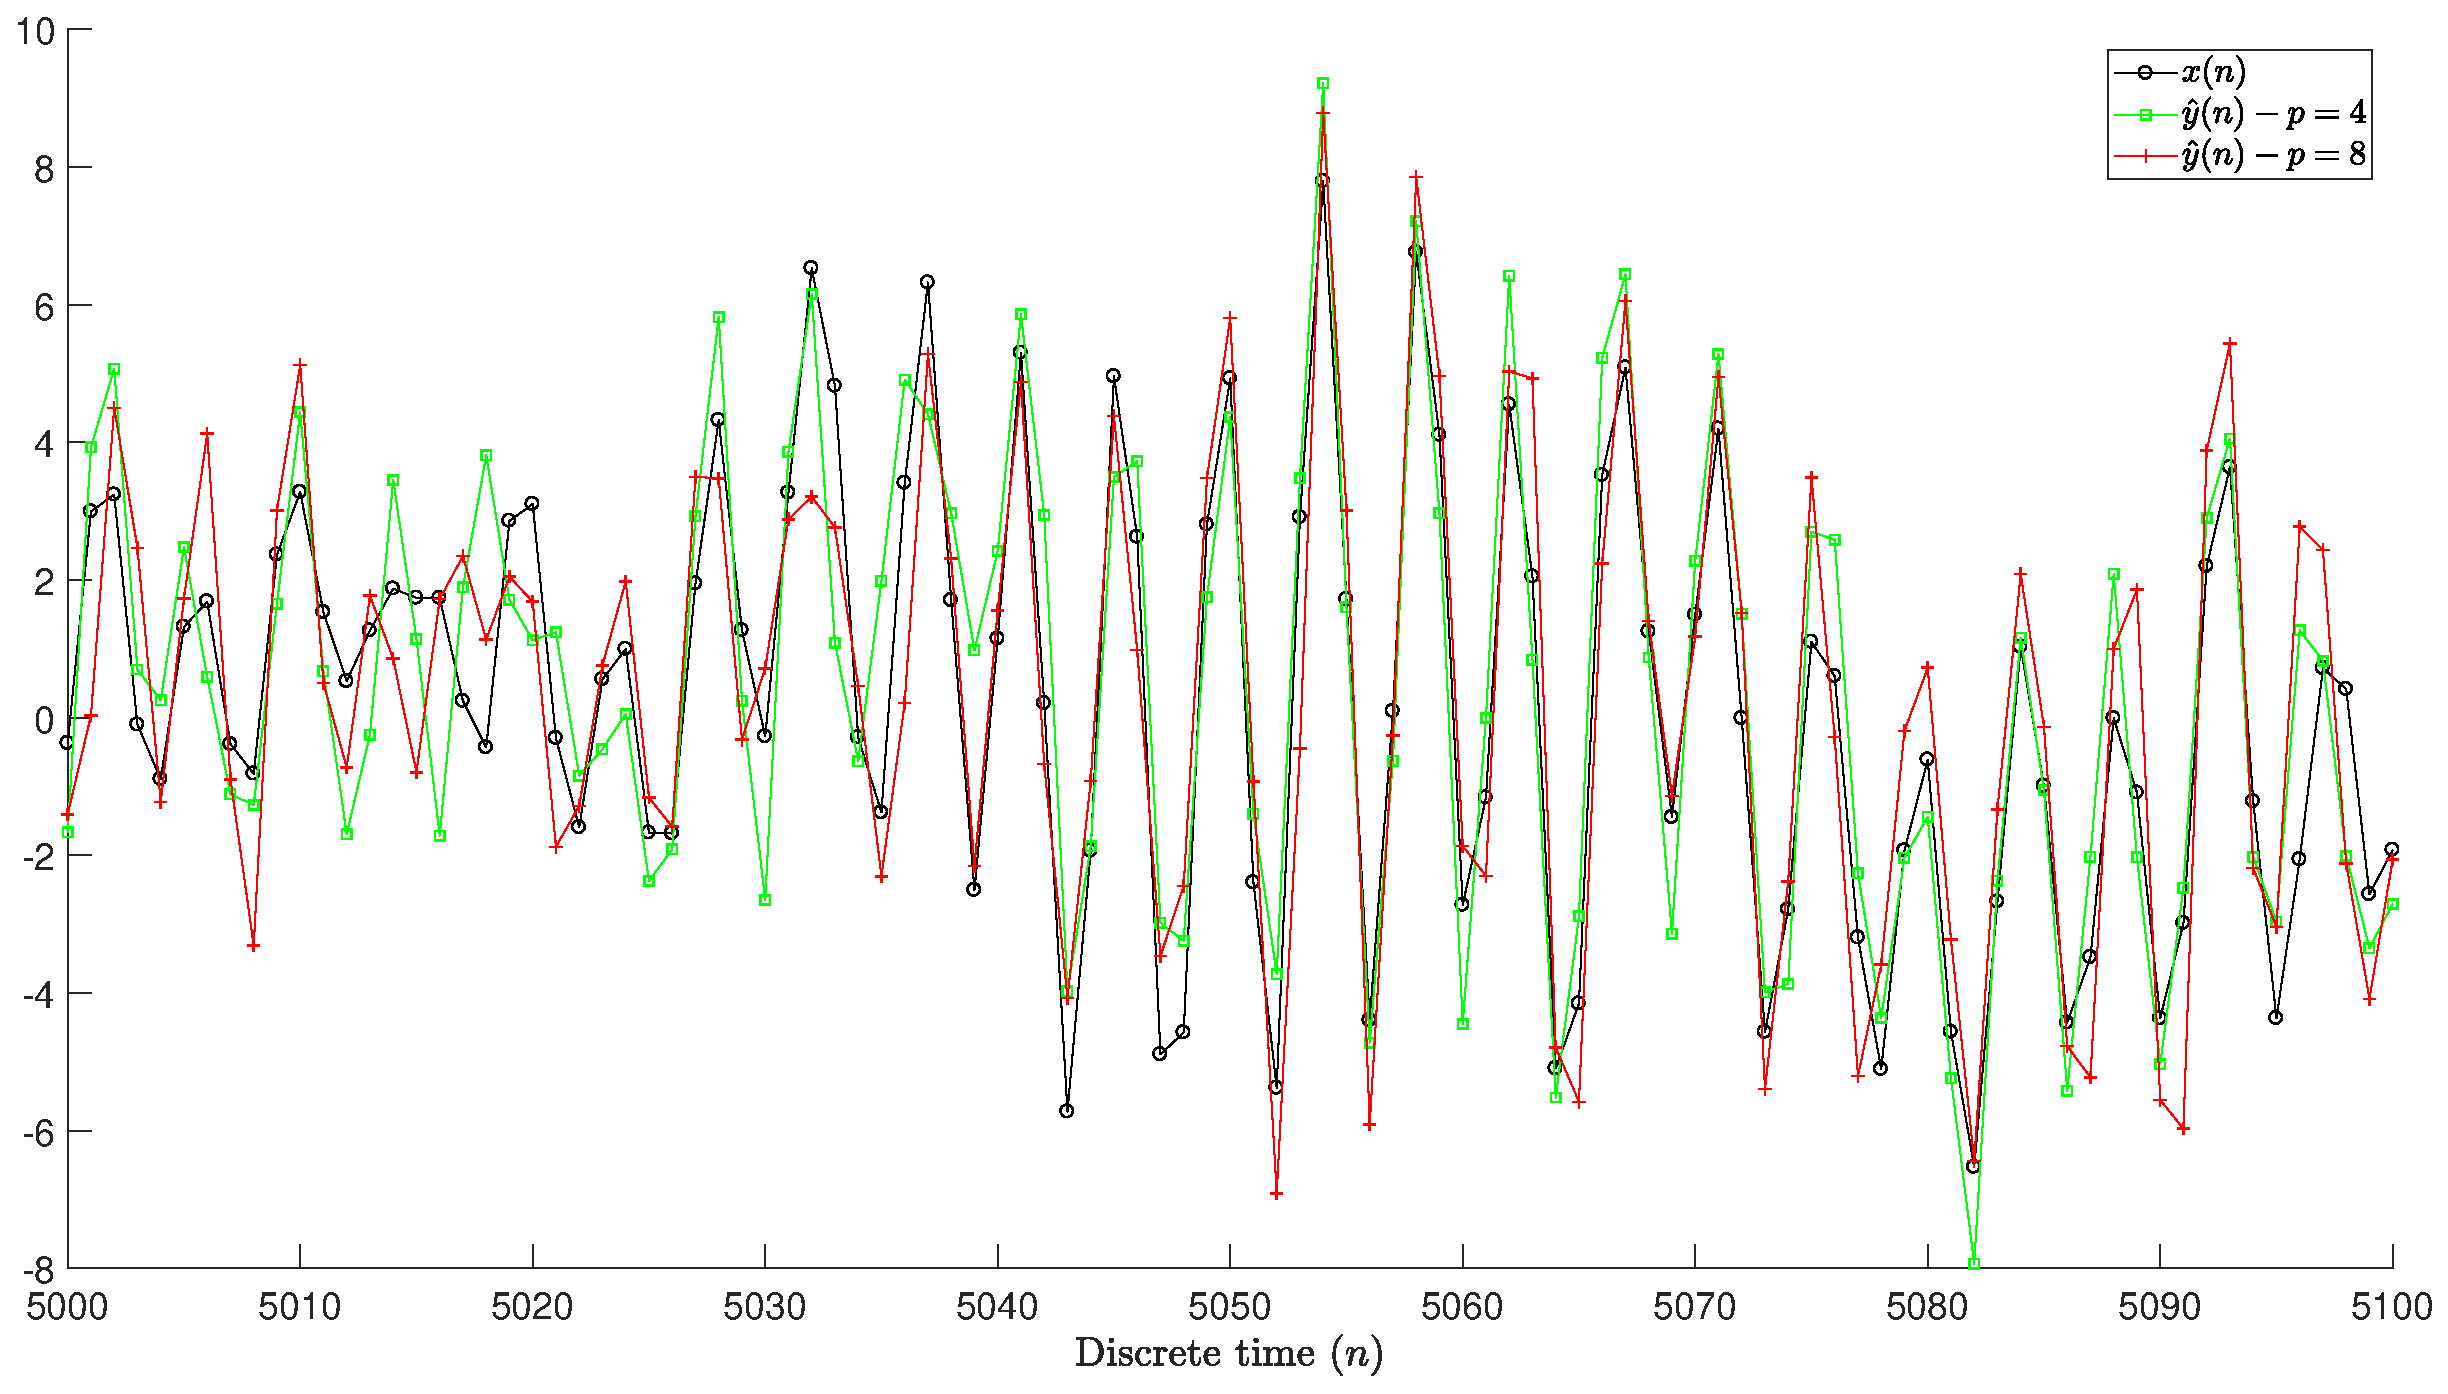
\includegraphics[width=0.95\textwidth, height = 5cm]{figures/dpcm_recon_N_1.eps}
            \caption{Διάγραμμα αρχικού και ανακατασκευασμένου σήματος και $Ν = 1$ \texten{bit}}
            \label{fig:dpcm_recon_N_1}
            \\\hspace{\textwidth}
            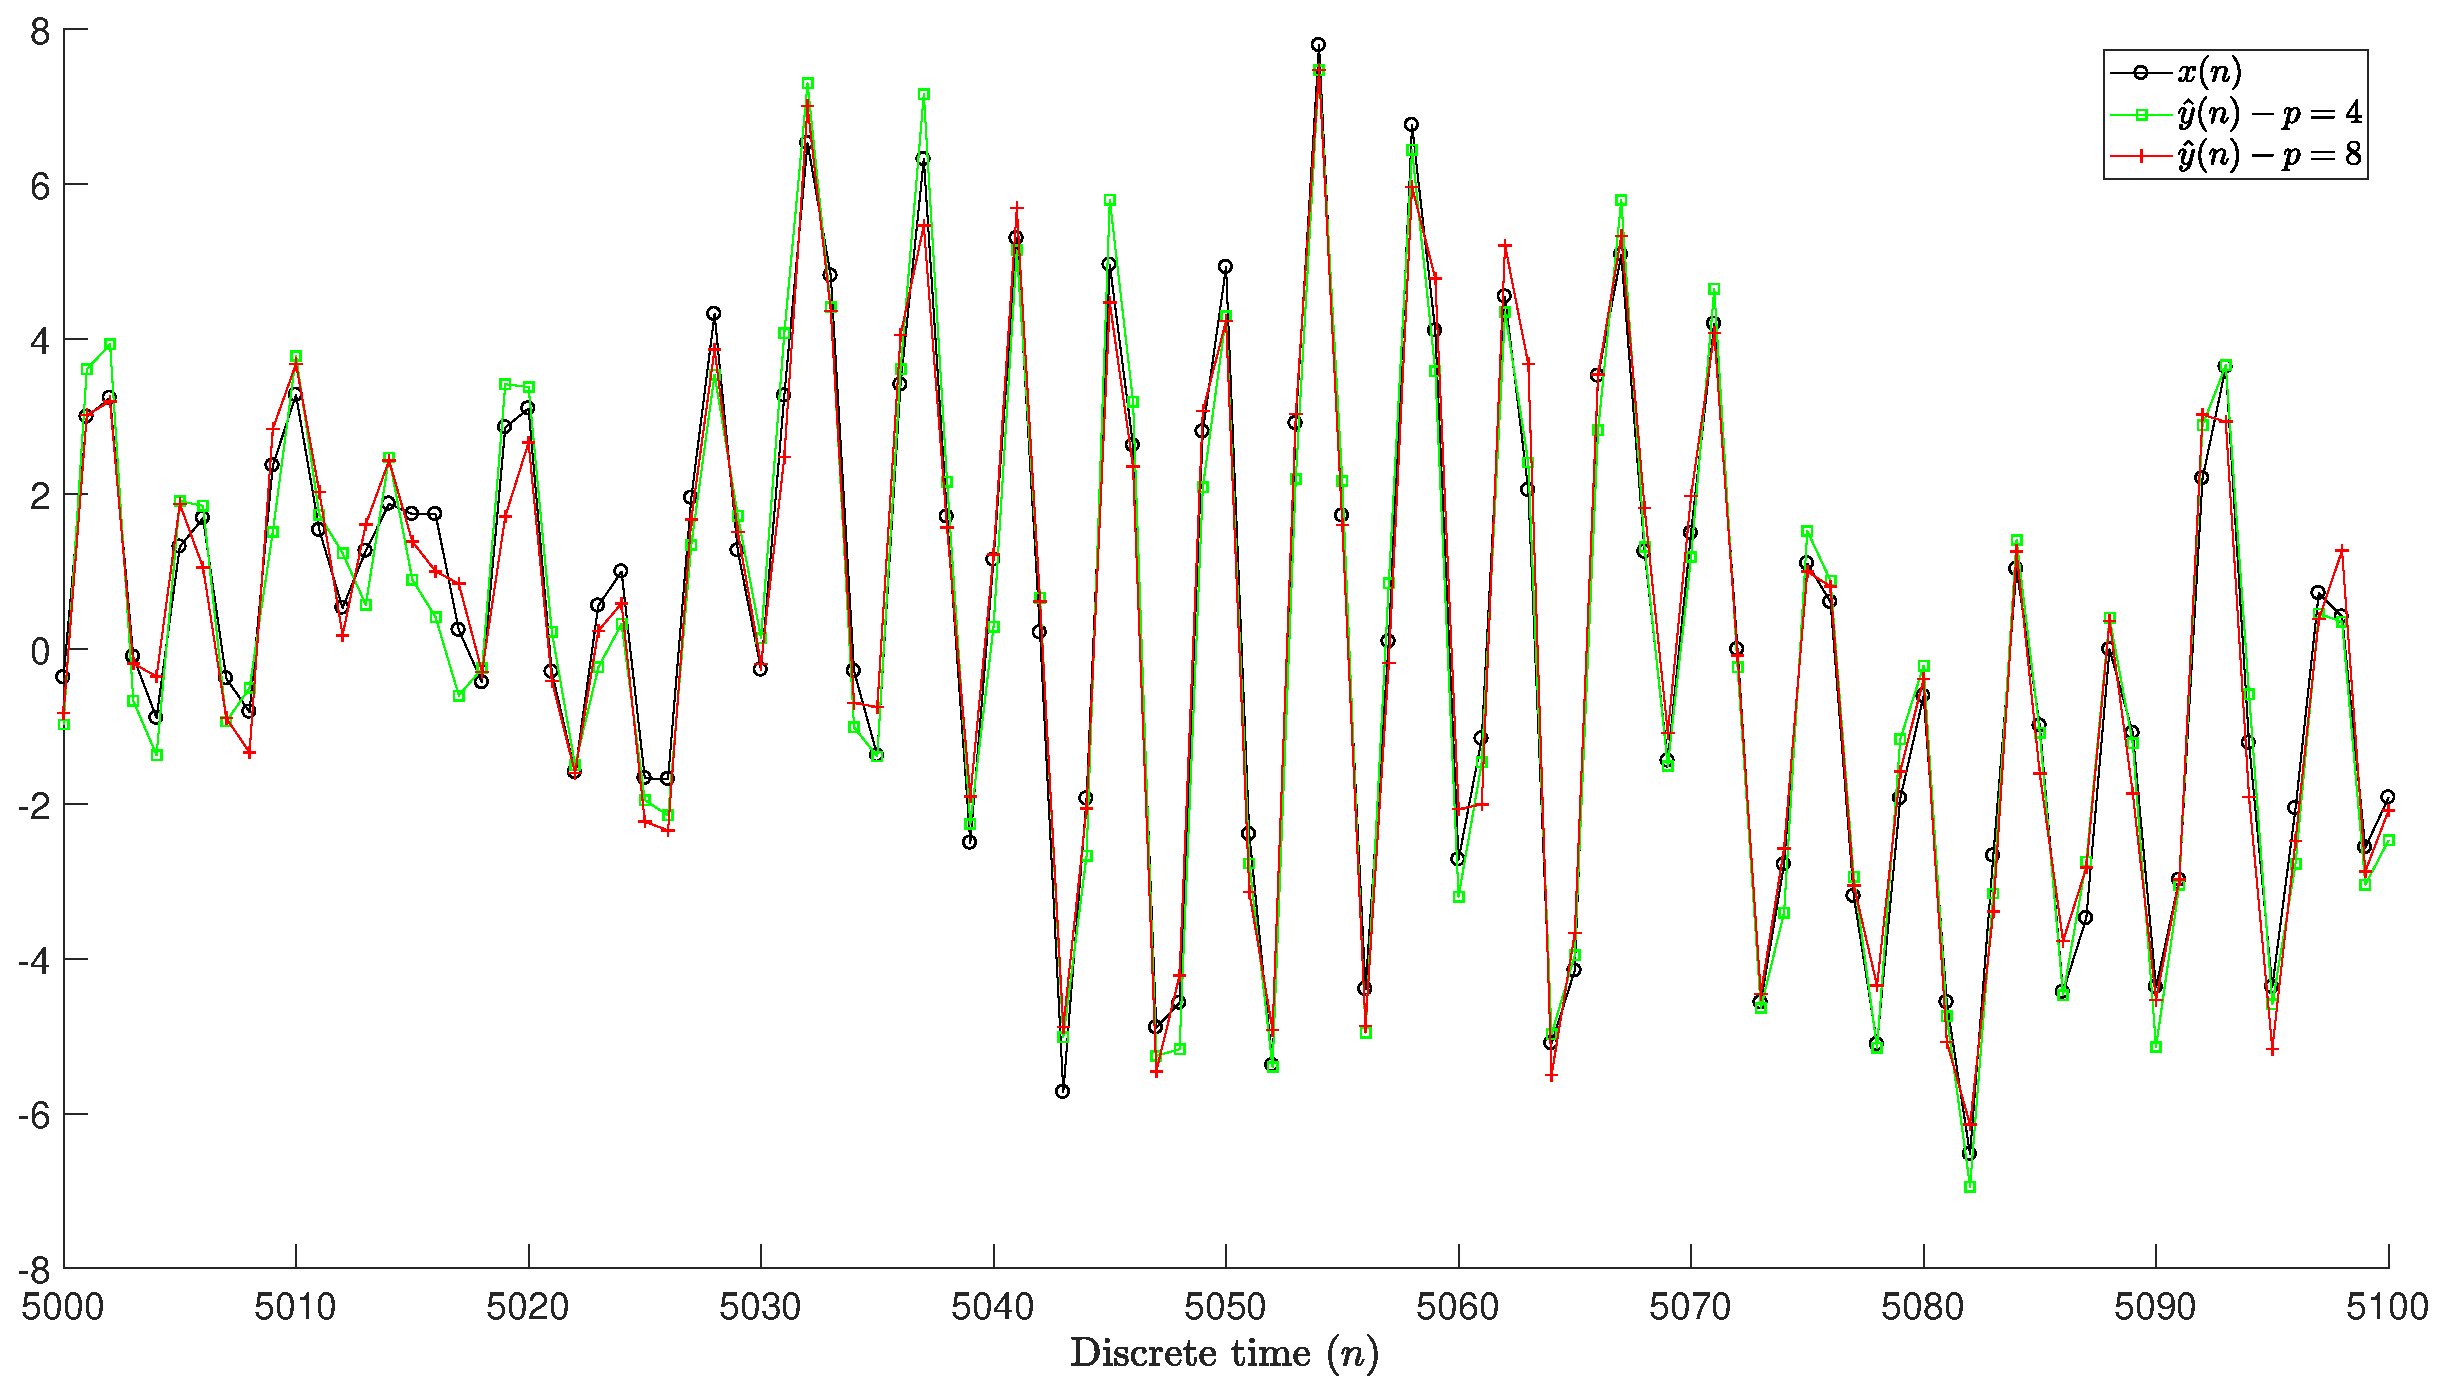
\includegraphics[width=0.95\textwidth, height = 5cm]{figures/dpcm_recon_N_2.eps}
            \caption{Διάγραμμα αρχικού και ανακατασκευασμένου σήματος και $Ν = 2$ \texten{bit}}
            \label{fig:dpcm_recon_N_2}
            \\\hspace{\textwidth}           
            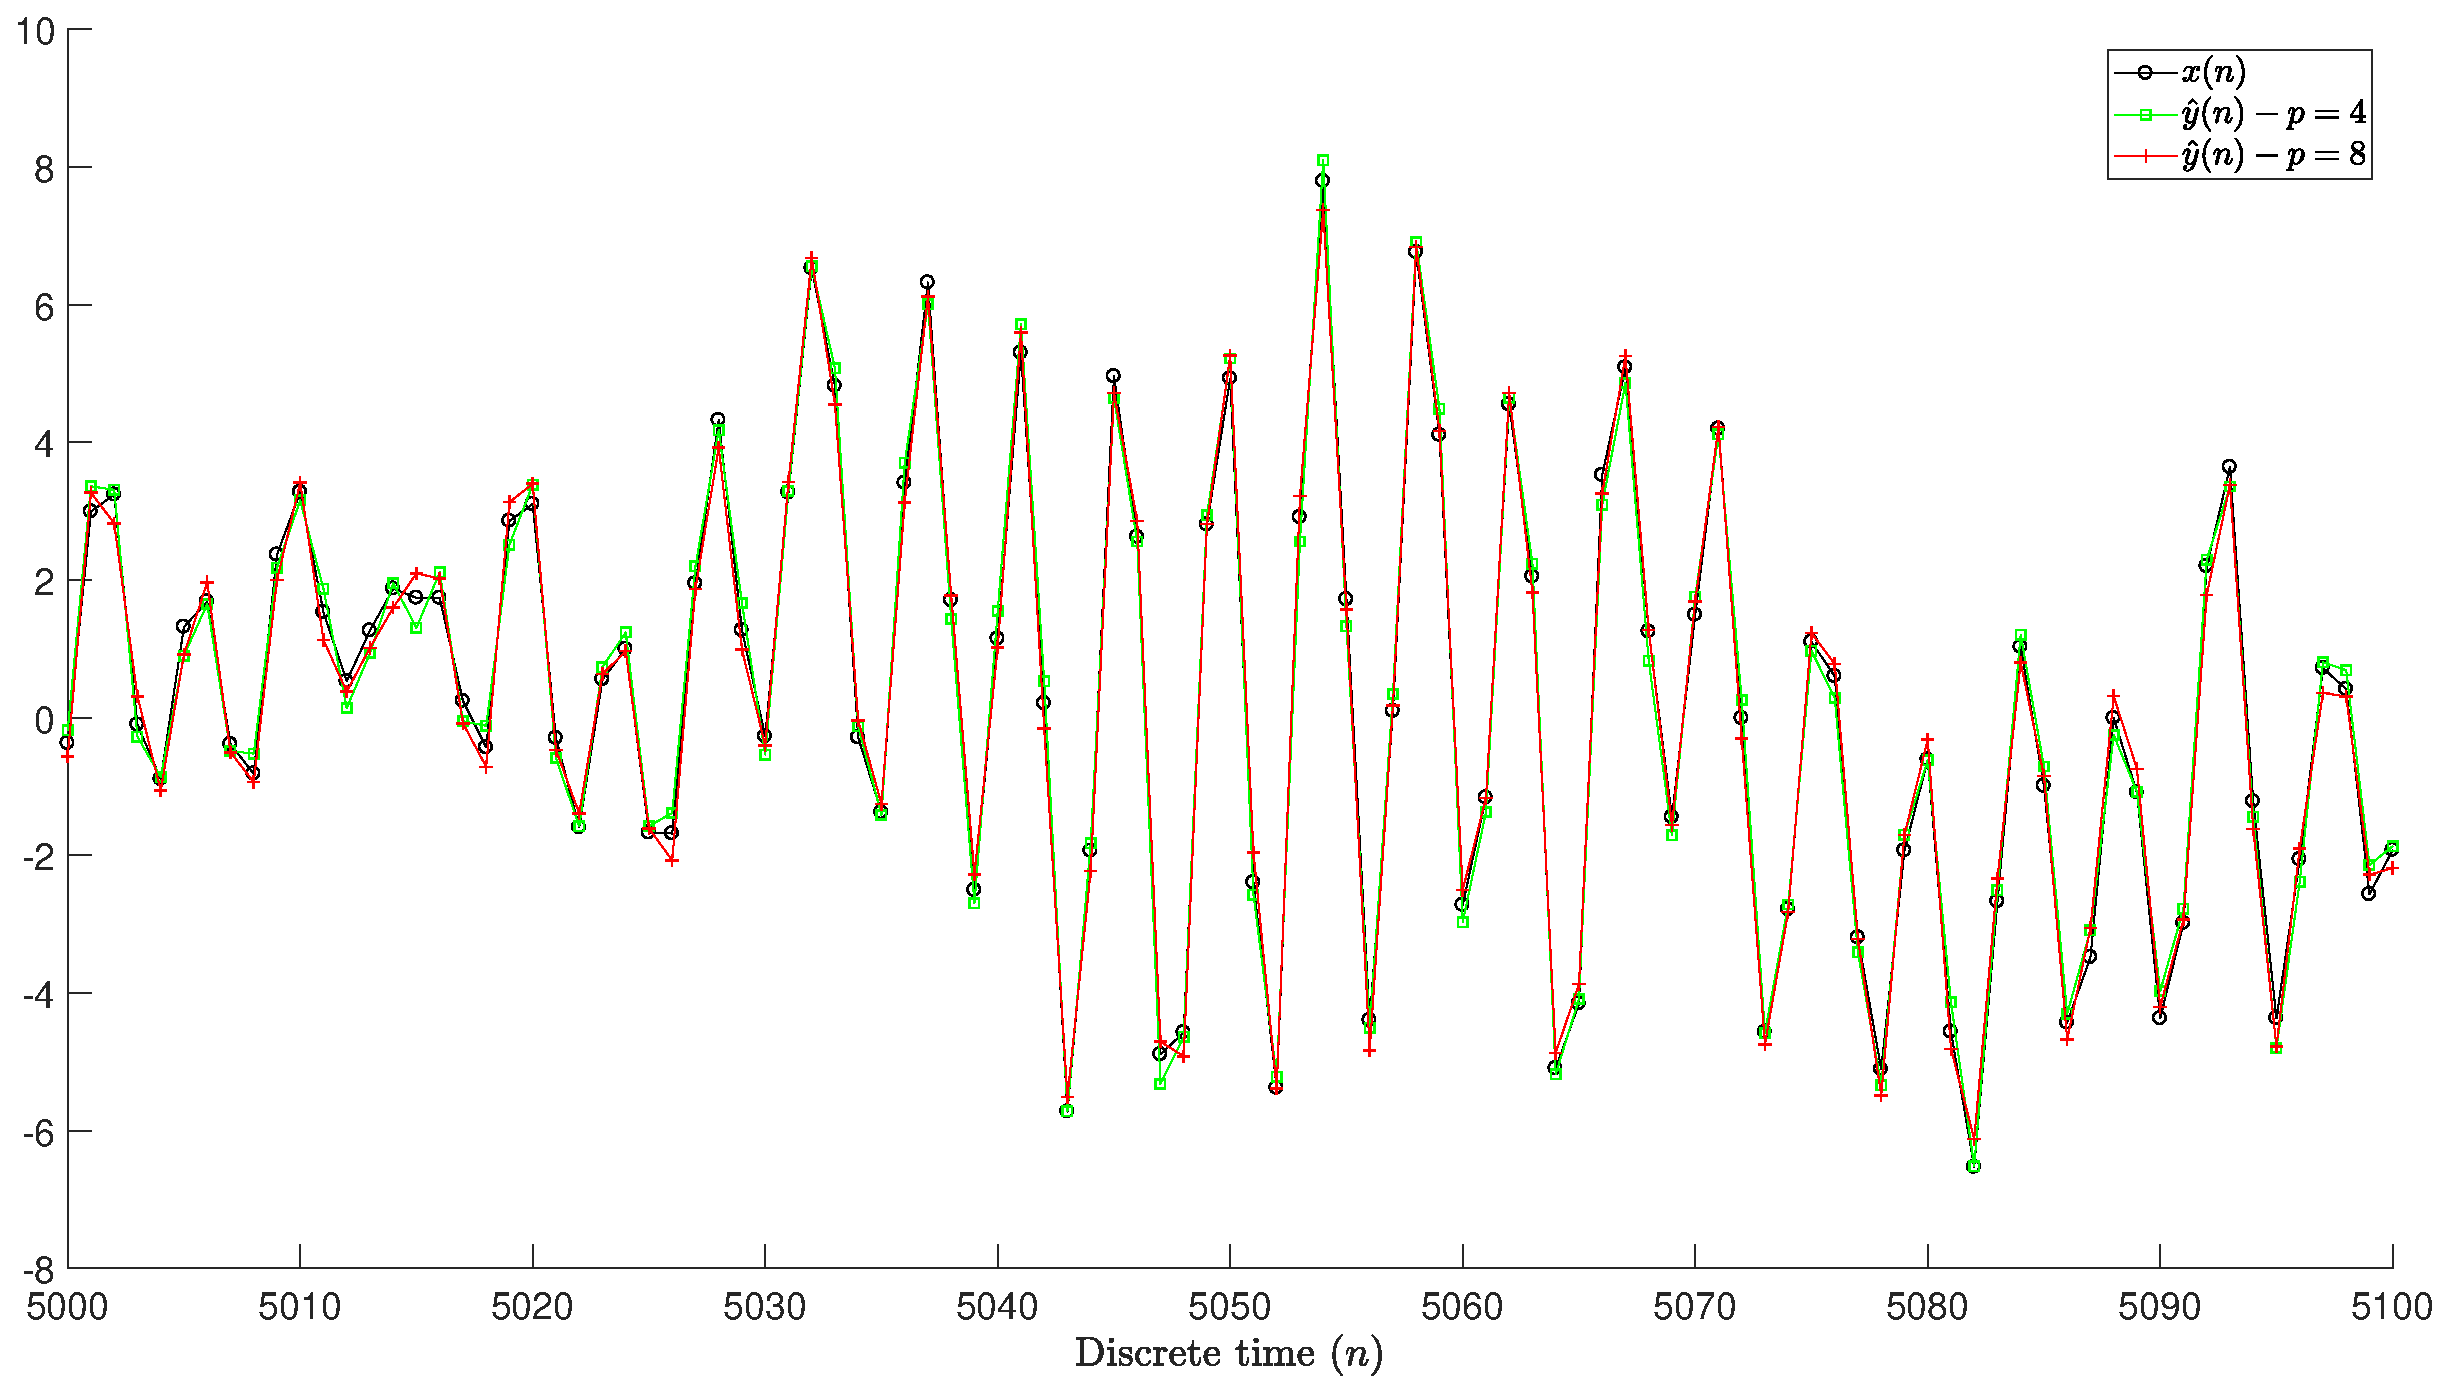
\includegraphics[width=0.95\textwidth, height = 5cm]{figures/dpcm_recon_N_3.eps}
            \caption{Διάγραμμα αρχικού και ανακατασκευασμένου σήματος και $Ν = 3$ \texten{bit}}
            \label{fig:dpcm_recon_N_3}
        \end{figure}        
        \\ Παρατηρώντας τις μετρήσεις γίνεται προφανές ότι όσα περισσότερα bits χρησιμοποιούνται τόσο
        καλύτερη είναι η ανακατασκεή του  αρχικού  σήματος. Αυτό επιβεβαιώνει και τα συμπεράσματα απο τα 
        προηγούμενα ερωτήματα, οτί μεγαλητερη  ακρίβεια κβάντισης μικρότερο σφάλμα πρόβλεψης.
    \newpage    
\begin{center} \section*{Παράρτημα Α} \end{center}
    \subsection*{ \underline{\texten{Matlab scripts \huff coding }} }
        \begin{itemize}
            \item[-] 
                \texttt{\texten{myHuffmanDict.m}}
                \texten{\lstinputlisting{matlab/huffman/myHuffmanDict.m}}
            \item[-] 
                \texttt{\texten{mySortStruct.m}}
                \texten{\lstinputlisting{matlab/huffman/mySortStruct.m}}
            \item[-] 
                \texttt{\texten{myHuffmanEnco.m}}
                \texten{\lstinputlisting{matlab/huffman/myHuffmanEnco.m}}
            \item[-] 
                \texttt{\texten{myHuffmanDeco.m}}
                \texten{\lstinputlisting{matlab/huffman/myHuffmanDeco.m}}
        \end{itemize}
    \newpage
    \subsection*{ \underline{Βοηθητικά \texten{Matlab scripts} για την επαλήθευση των 
    ερωτημάτων }}
        \begin{itemize}
        \item[-] 
            \texttt{\texten{random\_source\_test.m}}
            \texten{\lstinputlisting{matlab/huffman/test/random_source_test.m}}
        \item[-] 
            \texttt{\texten{kwords\_source\_test.m}}
            \texten{\lstinputlisting{matlab/huffman/test/kwords_source_test.m}}    
        \item[-] 
            \texttt{\texten{myFreqCompute.m}}
            \texten{\lstinputlisting{matlab/huffman/myFreqCompute.m}}
        \item[-] 
            \texttt{\texten{myNOrderSourceGen.m}}
            \texten{\lstinputlisting{matlab/huffman/myNOrderSourceGen.m}}
        \end{itemize}
\newpage
\newpage    
\begin{center} \section*{Παράρτημα B} \end{center}
    \subsection*{ \underline{\texten{Matlab scripts \dpcm }} }
        \begin{itemize}
        \item[-]      
            \code{my\_predictor\_factors.m}
            \texten{\lstinputlisting{matlab/dpcm/my_predictor_factors.m}}     
        \item[-]      
            \code{my\_quantizer.m}
            \texten{\lstinputlisting{matlab/dpcm/my_quantizer.m}}  
        \item[-]      
            \code{my\_dpcm\_trans.m}
            \texten{\lstinputlisting{matlab/dpcm/my_dpcm_trans.m}}  
        \item[-]      
            \code{my\_dpcm\_rec.m}
            \texten{\lstinputlisting{matlab/dpcm/my_dpcm_rec.m}}              
        \end{itemize}
    \subsection*{ \underline{Βοηθητικά \texten{Matlab scripts} για την επαλήθευση των 
    ερωτημάτων }}
        \begin{itemize}
        \item[-] 
            \code{dpcm\_predict\_test.m}
            \texten{\lstinputlisting{matlab/dpcm/dpcm_predict_test.m}}
        \item[-] 
            \code{dpcm\_mean\_square\_error.m}
            \texten{\lstinputlisting{matlab/dpcm/dpcm_mean_square_error.m}}       
        \item[-] 
            \code{dpcm\_reconstruct\_signal.m}
            \texten{\lstinputlisting{matlab/dpcm/dpcm_reconstruct_signal.m}}             
        \end{itemize}
\end{document}  

